
\documentclass[twocolumn]{article}

\usepackage{graphicx}
\usepackage{subfigure}

\begin{document}


\section{Experimental Results}

In this section, we empirically evaluate the performance of proposed online heterogeneous transfer learning algorithms and classic online Passive-Aggressive algorithms (PA).
Encouraging results demonstrate that the proposed algorithms outperform these algorithms.

% dataset & task description
\subsection{Dataset}
Our experiments are conducted for image classification by leveraging information from text data.
We use NUS-WIDE dataset to generate learning tasks.
The NUS-WIDE dataset is extracted from Flickr.
It includes 269,648 images and the associated tags from Flickr, with a total number of 5,018 unique tags.
An image instance is represented by a feature vector based on SIFT descriptions, and a text instance is represented by a feature vector based on tags.
There are 81 ground-truth class labels in the dataset.
We randomly selected 10 classes (bird, boat, car, flower, food, rock, sun, toy, tree) and built $C_{10}^{2} = 45$ binary classification tasks.

We refer the images as data in the target domain, and the tags as the text data in the heterogeneous source domain.
Each binary classification task has 500 image instances in the target domain, 1,200 text instances in the heterogeneous source domain, and 1,500 co-occurred image-text pairs.
In order to obtain stable results, we draw 100 times of random permutation of the image instances in the target domain and evaluate the performance of learning algorithms based on mean and standard deviation of mistake rates.

% methods to be compared
% experimental setup 
%   kernel function
%   parameters setting
%   parameter sensitivity
%   times
%   evaluation metric

\subsection{Baseline Methods}
We compare the proposed methods with Passive-Aggressive (PA) online learning algorithms.
PA algorithm proposed by Crammer et al. does not exploit knowledge from the source domain.
It deals with the traditional online learning problem in the target domain.

For fair comparison and simplicity, we adopt Gaussian kernel function in all the algorithms and tasks.
The kernel parameter $\sigma = 8$ for the target domain.
The regularization parameter $C = 5$, $ \beta = \frac{\sqrt{T}}{\sqrt{T}+\sqrt{2\ln{4}}} $ for OHT-II algorithm.
In addition, we set the number of nearest neighbors to be considered $K = 10$.
Sensitivity of parameters will be examined in subsequent sections.

\subsection{Results and Discussion}

% figures of mean mistake rates
% tables of mean and standard derivation of mistake rates
% significant test results
% Cohen's d
\begin{figure*}[!htb]
\begin{center}
  \subfigure[PA vs OHT1]
  {
    \label{fig:subfig:a}
    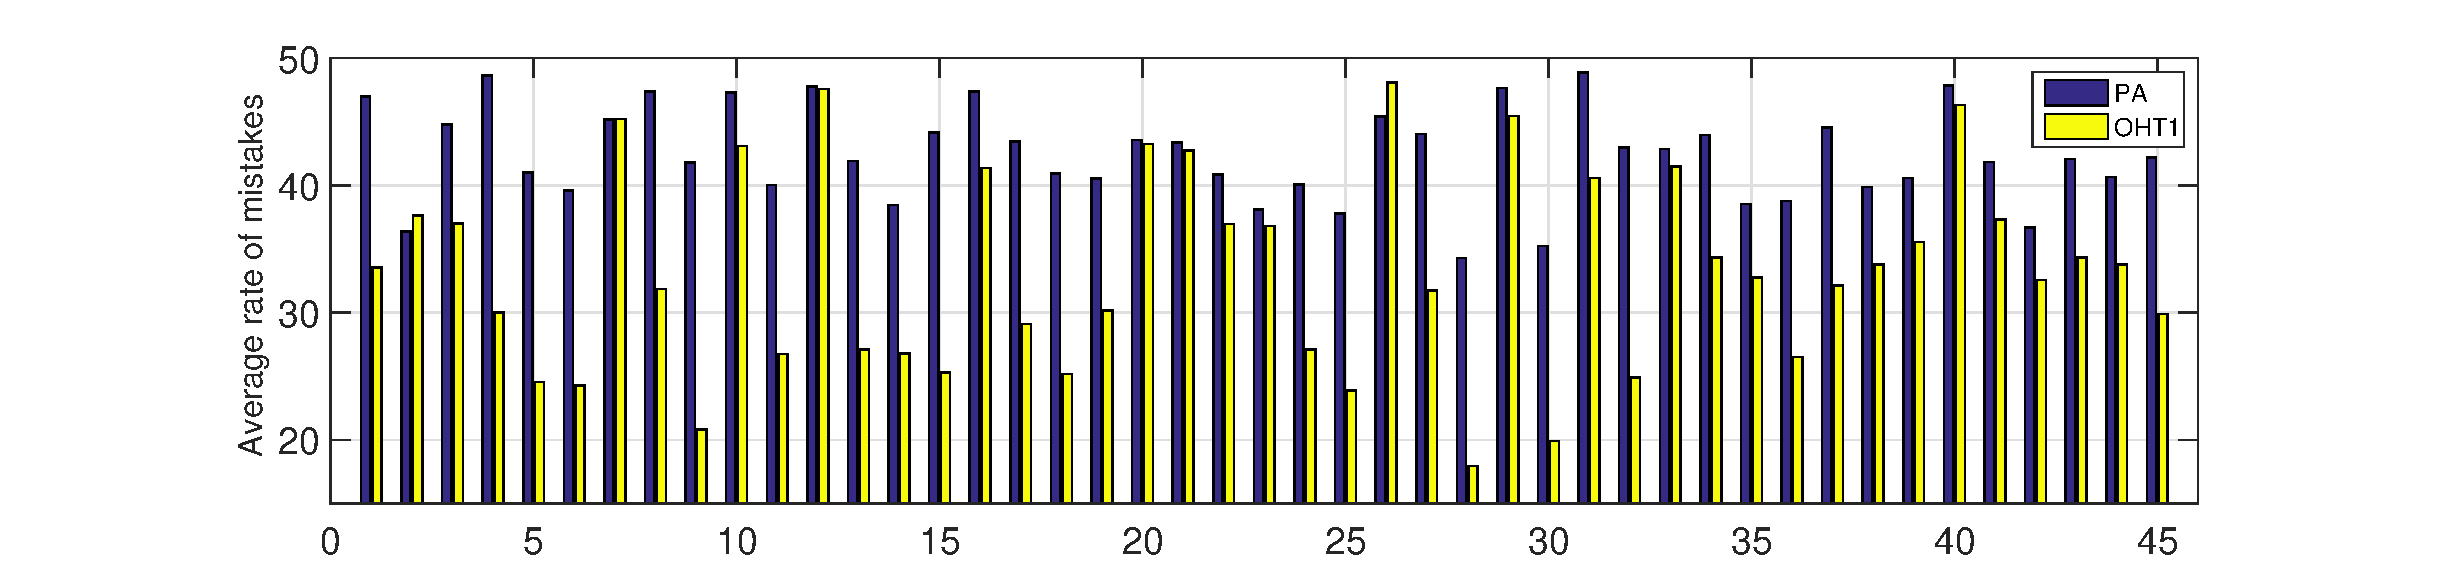
\includegraphics[width=18cm]{11.eps}
  }
  \subfigure[PA vs OHT2]
  {
    \label{fig:subfig:b}
    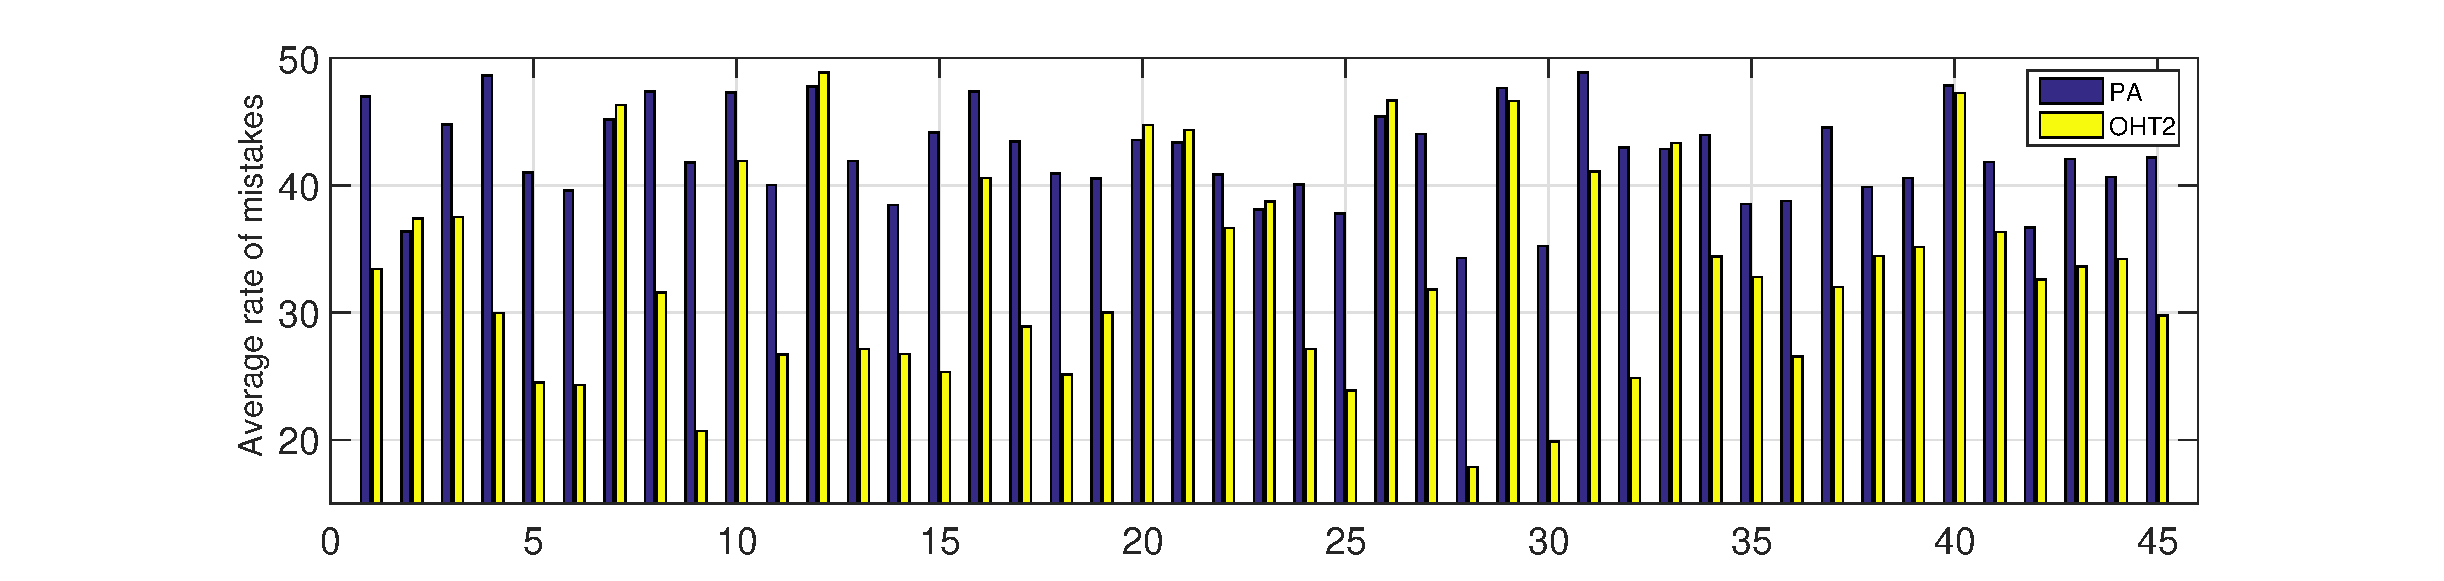
\includegraphics[width=18cm]{12.eps}
  }
\end{center}
  \caption{Results on all 45 tasks}
  \label{Results}
\end{figure*}

Table summarizes the mistake rates of all 45 tasks.
We see that in most tasks, PA has the very high mistake rate, which prove the dificulty of image classification task without any auxiliary source information.
The observation that our proposed OHT algorithms generally outperform PA validates the effectivity of heterogeneous transfer.

Figure illustrates the dynamic process of several online learning tasks, respectively.
We observe that in some tasks(e.g., 35, 39 and 41), the mistake rates of all three algorithms decrease during the period, and OHT algorithms always achieve better performance than PA.
Furthermore, in some tasks(e.g., 8, 11 and 24), OHT algorithms are able to obtain a good performance at the beginning stage and remain stable in the future.
These observations verifies that the OHT algorithms indeed transfer useful knowledge from the heterogeneous source domain to the target domain. 

\begin{figure*}[!htb]
\begin{center}
  \subfigure[Task 8]
  {
    \label{fig:subfig:a}
    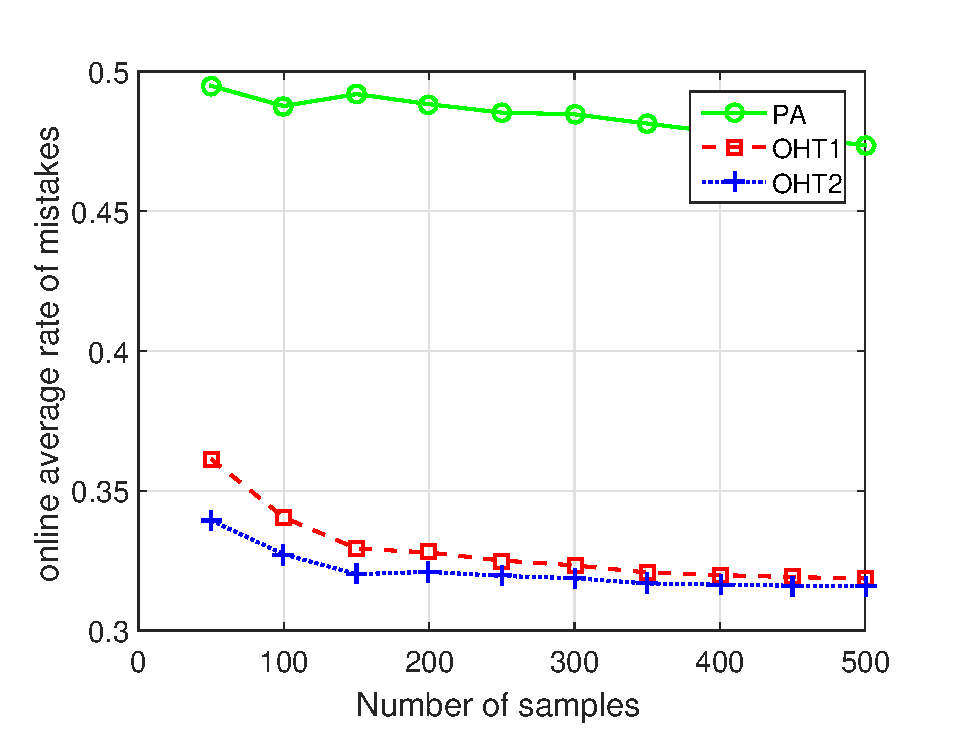
\includegraphics[width=5cm]{task8.eps}
  }
  \subfigure[Task 11]
  {
    \label{fig:subfig:b}
    \includegraphics[width=5cm]{task11.eps}
  }
  \subfigure[Task 24]
  {
    \label{fig:subfig:c}
    \includegraphics[width=5cm]{task24.eps}
  }
  \\
  \subfigure[Task 35]
  {
    \label{fig:subfig:d}
    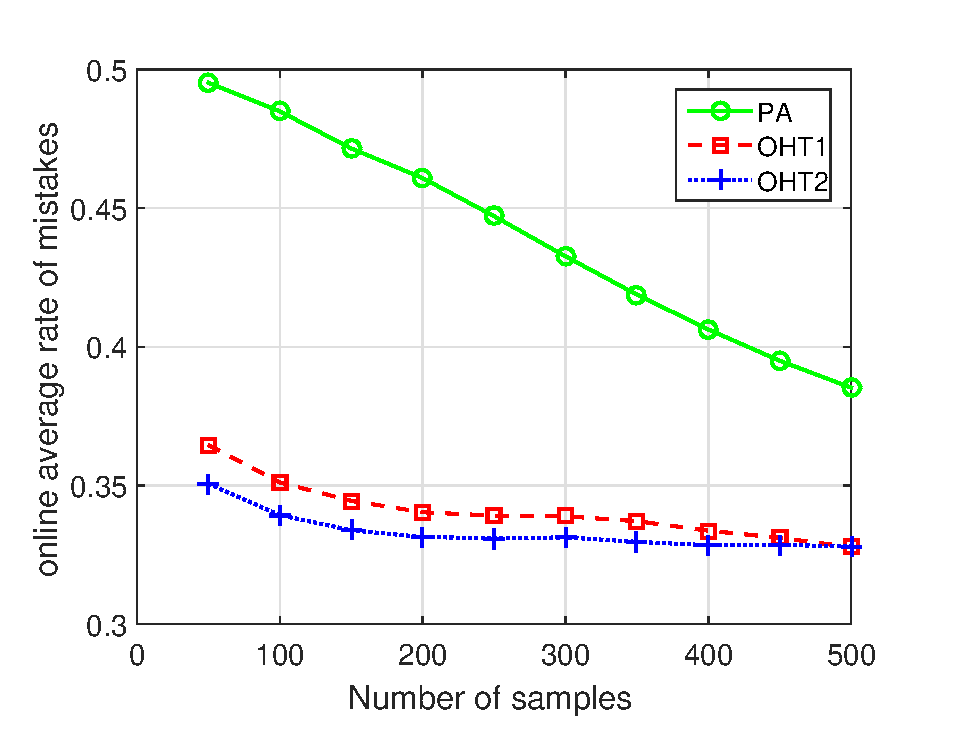
\includegraphics[width=5cm]{task35.eps}
  }
  \subfigure[Task 39]
  {
    \label{fig:subfig:e}
    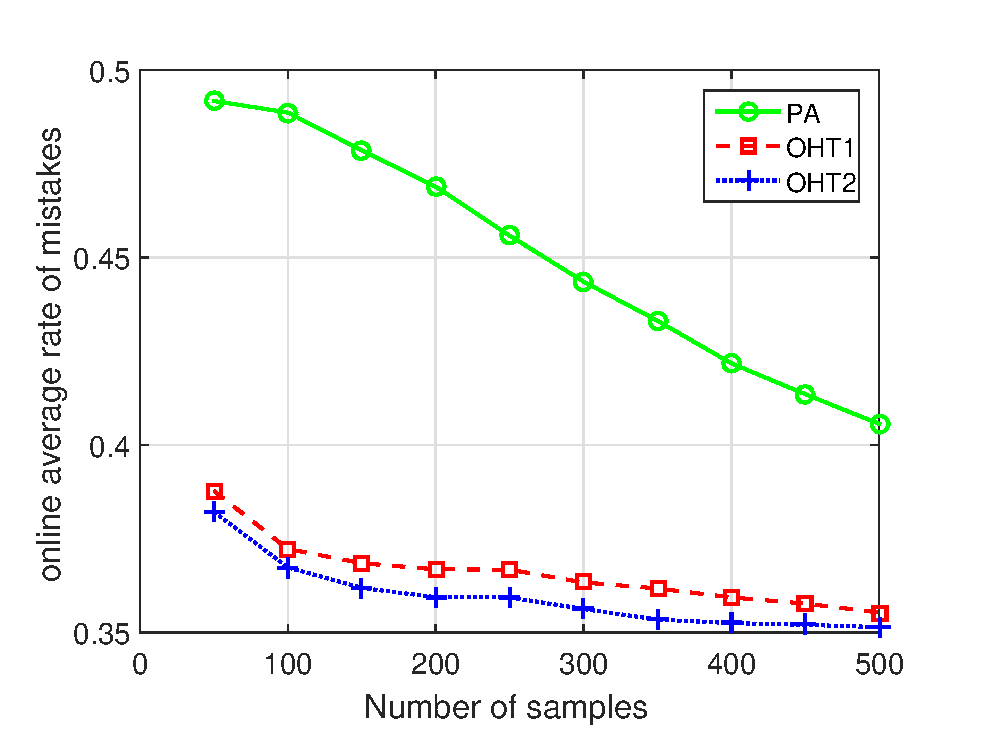
\includegraphics[width=5cm]{task39.eps}
  }
  \subfigure[Task 41]
  {
    \label{fig:subfig:f}
    \includegraphics[width=5cm]{task41.eps}
  }
  
  \caption{Online mistake rates}
  \label{Online mistake rates}
\end{center}
\end{figure*}

We also analyze the performance difference between PA and two OHT algorithms.
Statistical significance against PA was assessed by paired $t$-test at 0.05 level.
For each task, a win (or loss) is counted when OHT algorithm is significatly better (or worse) than PA algorithm over 100 trials.
Otherwise, a tie is recorded.
The win/tie/loss results is 30/1/1 for competition between OHT1 and PA, and 30/1/1 for competition between  OHT2 and PA.
This result validates that our OHT algorithms is statistically better than PA algorithm.

Besides, we make use of Cohen's $d$ value to measure the improvement of our algorithms.
$d >= 0.8$ generally indicates a large promotion.
OHT1 algorithm achieves large improvement in 30 tasks and middle improvement in 3 tasks.
For OHT2 algorithms, the numbers are 32 and 2.

\subsection{Parameters and Running time}
% parameter sensitivity
\paragraph{Parameters}
Experiments in paper about online transfer learning illustrated that the performance of online transfer learning algorithms is generally insensitive to the parameter C and $\beta$.
Therefor, we only investigate how different values of parameter K affect the classification accuracy of the algorithms.
We select a number of tasks randomly to evaluate the parameter sensitivity.
Table shows the performance of the proposed algorithms with varied values of parameter K in task 1.
We observe that the performance of the algorithms is stable.
Similar obvervation are showed in other tasks.
In consideration of that we employ the weighted K nearest neighbors strategy, it is easy to understand.
The larger distance a instance in the heterogeneous source domain has, the less impact the instance makes.


% running time
\paragraph{Running time}
Table shows the mean and standard deviation of running time of different algorithms in several randomly selected tasks.
All of the algorithms were implemented in Matlab, and all experiments were run in a Linux machine with 3.2 GHz CPU and 3.8 GB memory.
From the table, we can see that PA without exploiting knowledge from the source domain is the most efficient.
Two OHT algorithms are less efficient.
The main reason of more running time is the searching process for the nearest neighbors.
Because of the insensitivity of parameter $K$, we can simply make use of all instances in the heterogeneous source domain to decrease the running time and obtain comparable performance.



\end{document}
